% Chapter Analysis Strategy

\chapter{Systematic Uncertainty} \label{chap:5}

\section{Systematic Uncertainty on Signal Selection} 

\begin{itemize}
%CMS-PAS-LUM-17-001
  \item Luminosity: Integrated luminosity is estimated with 2.5$\% $ uncertainty~\citep{CMS-PAS-LUM-17-001}. 
  \item Pile-ups: Pile-up efficiency scale factor is applied to simulation weight the pile-up distribution as that of data. The pile-up distribution of data is measured by assuming minibias cross section equals to 69.2 mb, which has 4.6$\% $ uncertainty. 
  \item Higgs tagging: Since there is no pure Higgs events in data, we cannot obtain the scale factor of Higgs-get tagging using the data. Instead, the Higgs-tagged uncertainty is measured by Higgs-jets and W-jets from simulation. The difference in mass scale and their jet flavor composition lead to different hadron shower response. Two shower and hadronization models is used to see how the hadronization effects the jet tagging. The bulk graviton $\rightarrow$ WW and bulk graviton $\rightarrow$ HH are used for the W-jets and Higgs-jets respectively. First, we calculate the efficiency of both jets in two models: PYTHIA and  HERWIG. Then, for each model, we divide the $\varepsilon_{HH}$ by $\varepsilon_{WW}$ to get the efficiency ratio, referred as R. Finally, the systematic uncertainty is derived from the uncertainty of double ratio R$_{HERWIG}$/R$_{PYTHIA}$. There is $p_{T}$ dependent uncertainty by fitting to the uncertainties of different mass point, which gives overall 13 to 19 $\% $ uncertainty~\citep{AN-16-300}.
  
  
\begin{figure}[t]
  \centering
 \begin{tabular}{cc}
    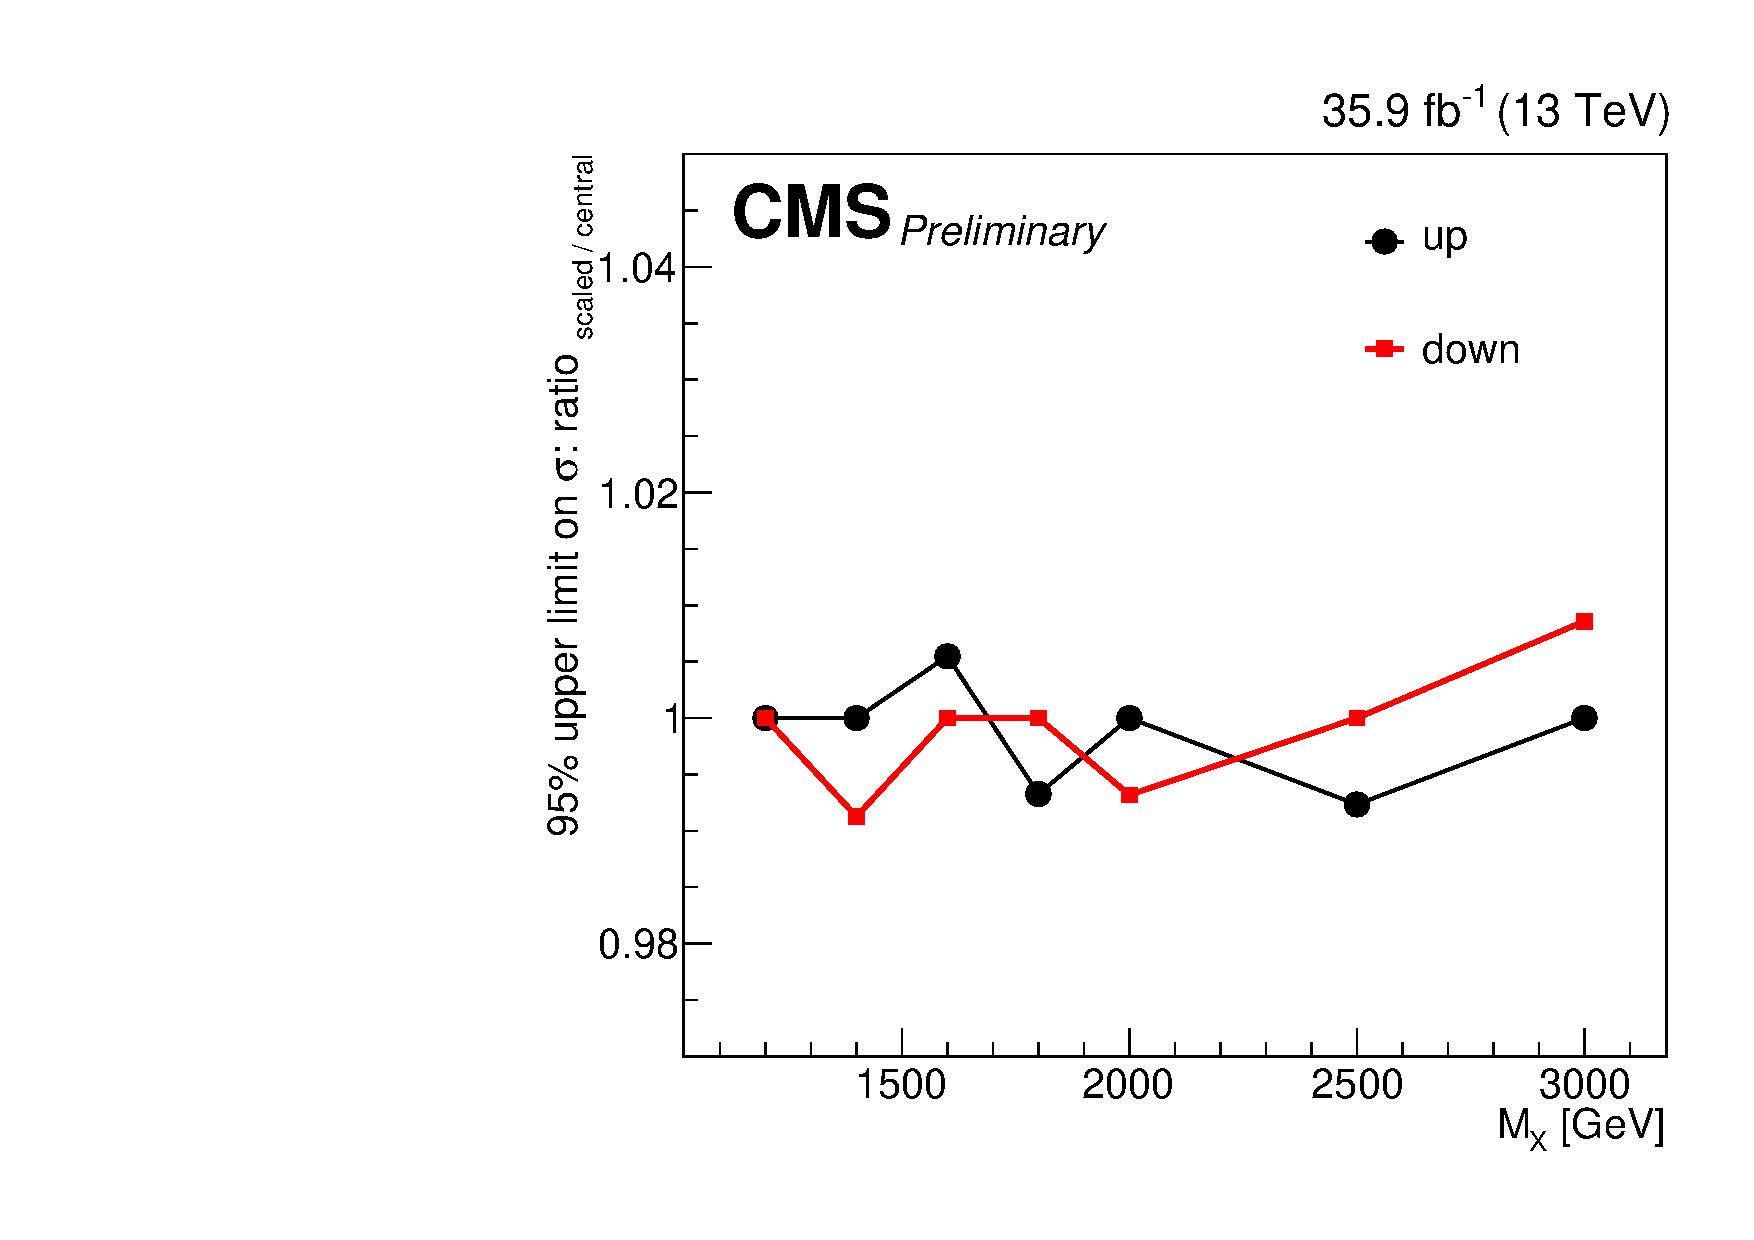
\includegraphics[width=0.5\textwidth]{Figures/plots_uncert/pu_TT.pdf} &
   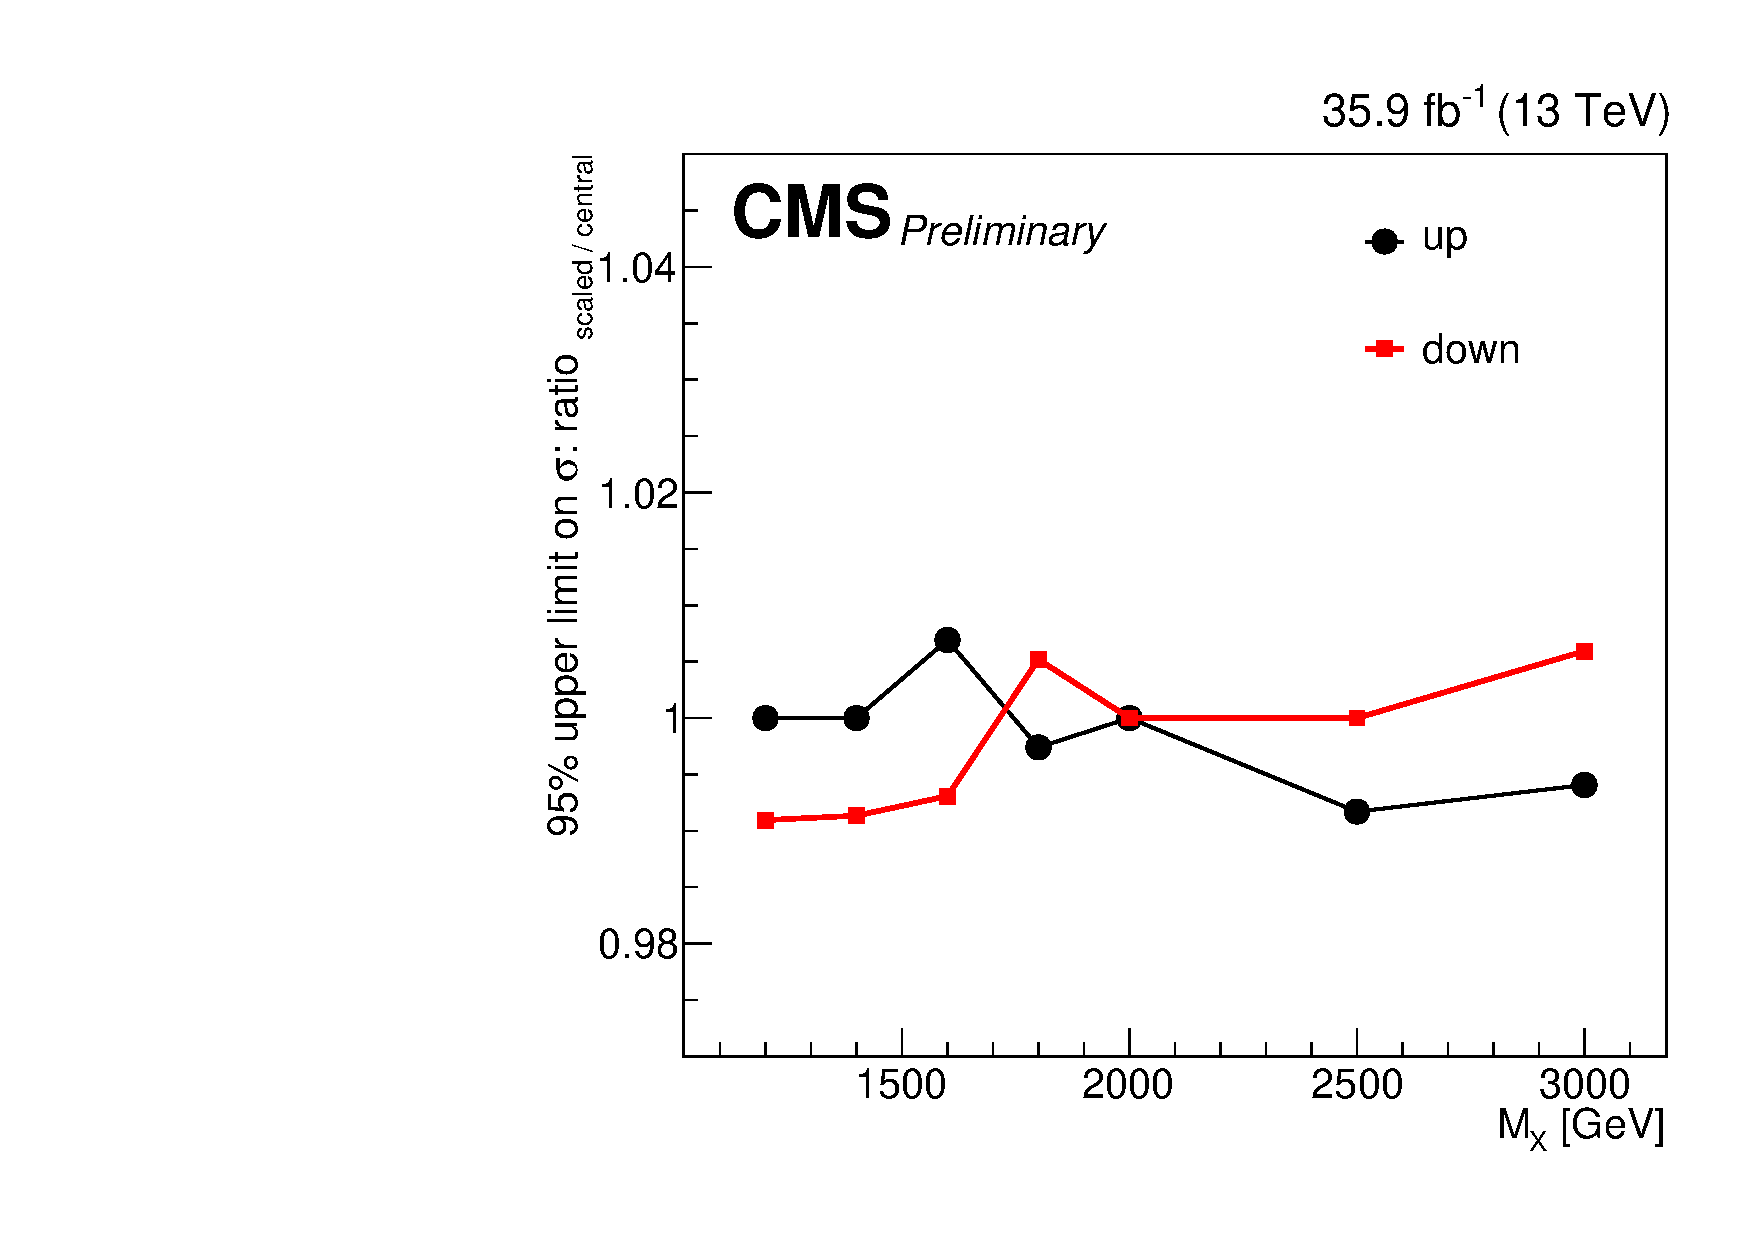
\includegraphics[width=0.5\textwidth]{Figures/plots_uncert/pu_LL.pdf} \\
  \end{tabular}
  \caption{The pile-up uncertainty. The scale-up and scale-down to central ratio based on the change of the upper limit are shown in TT (left) and LL (right) category.}

\end{figure}  
   
  \item Double-b tagger scale factor: The double-b tagger scale factor and its uncertainty is provided by BTV POG~\citep{BtagRecommendation80XReReco}.
  
\begin{figure}[t]
  \centering
 \begin{tabular}{cc}
    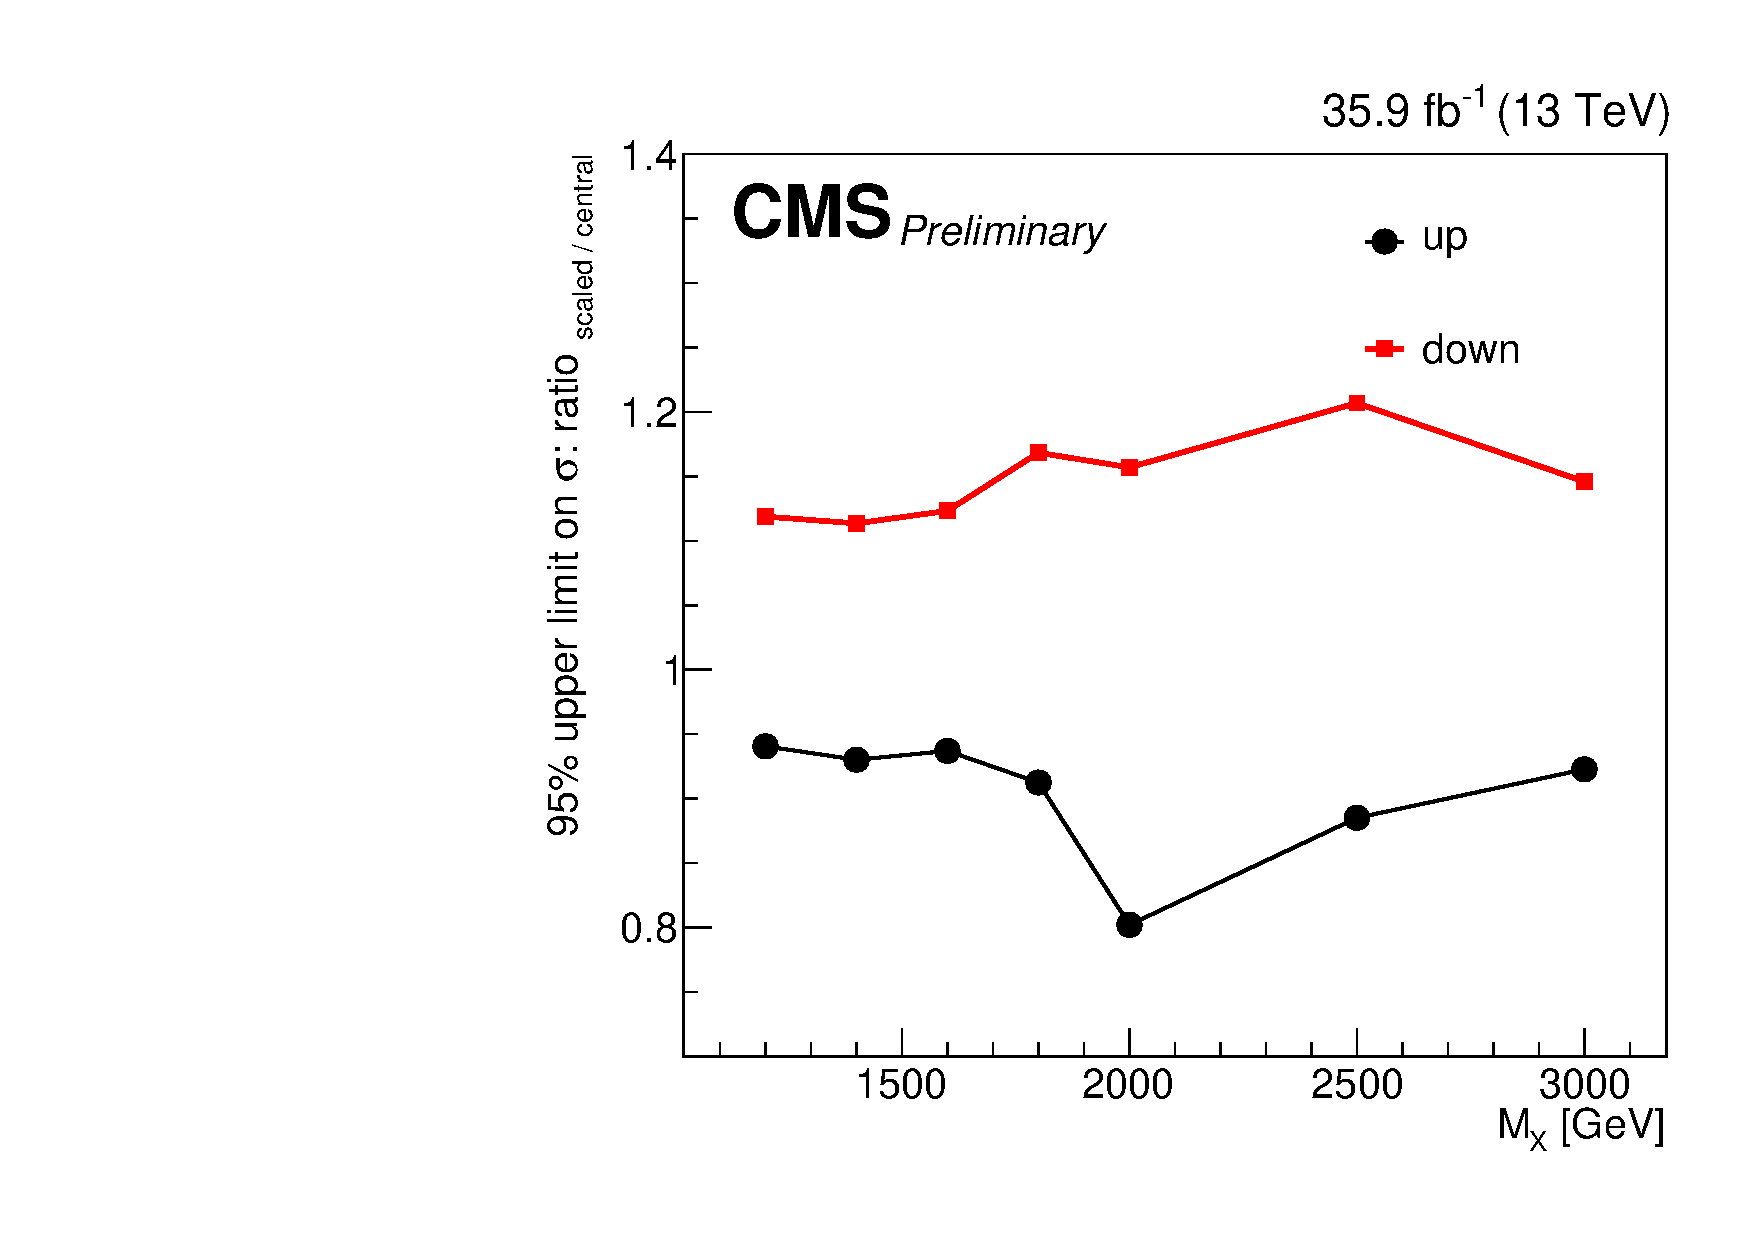
\includegraphics[width=0.5\textwidth]{Figures/plots_uncert/btag_TT.pdf} &
   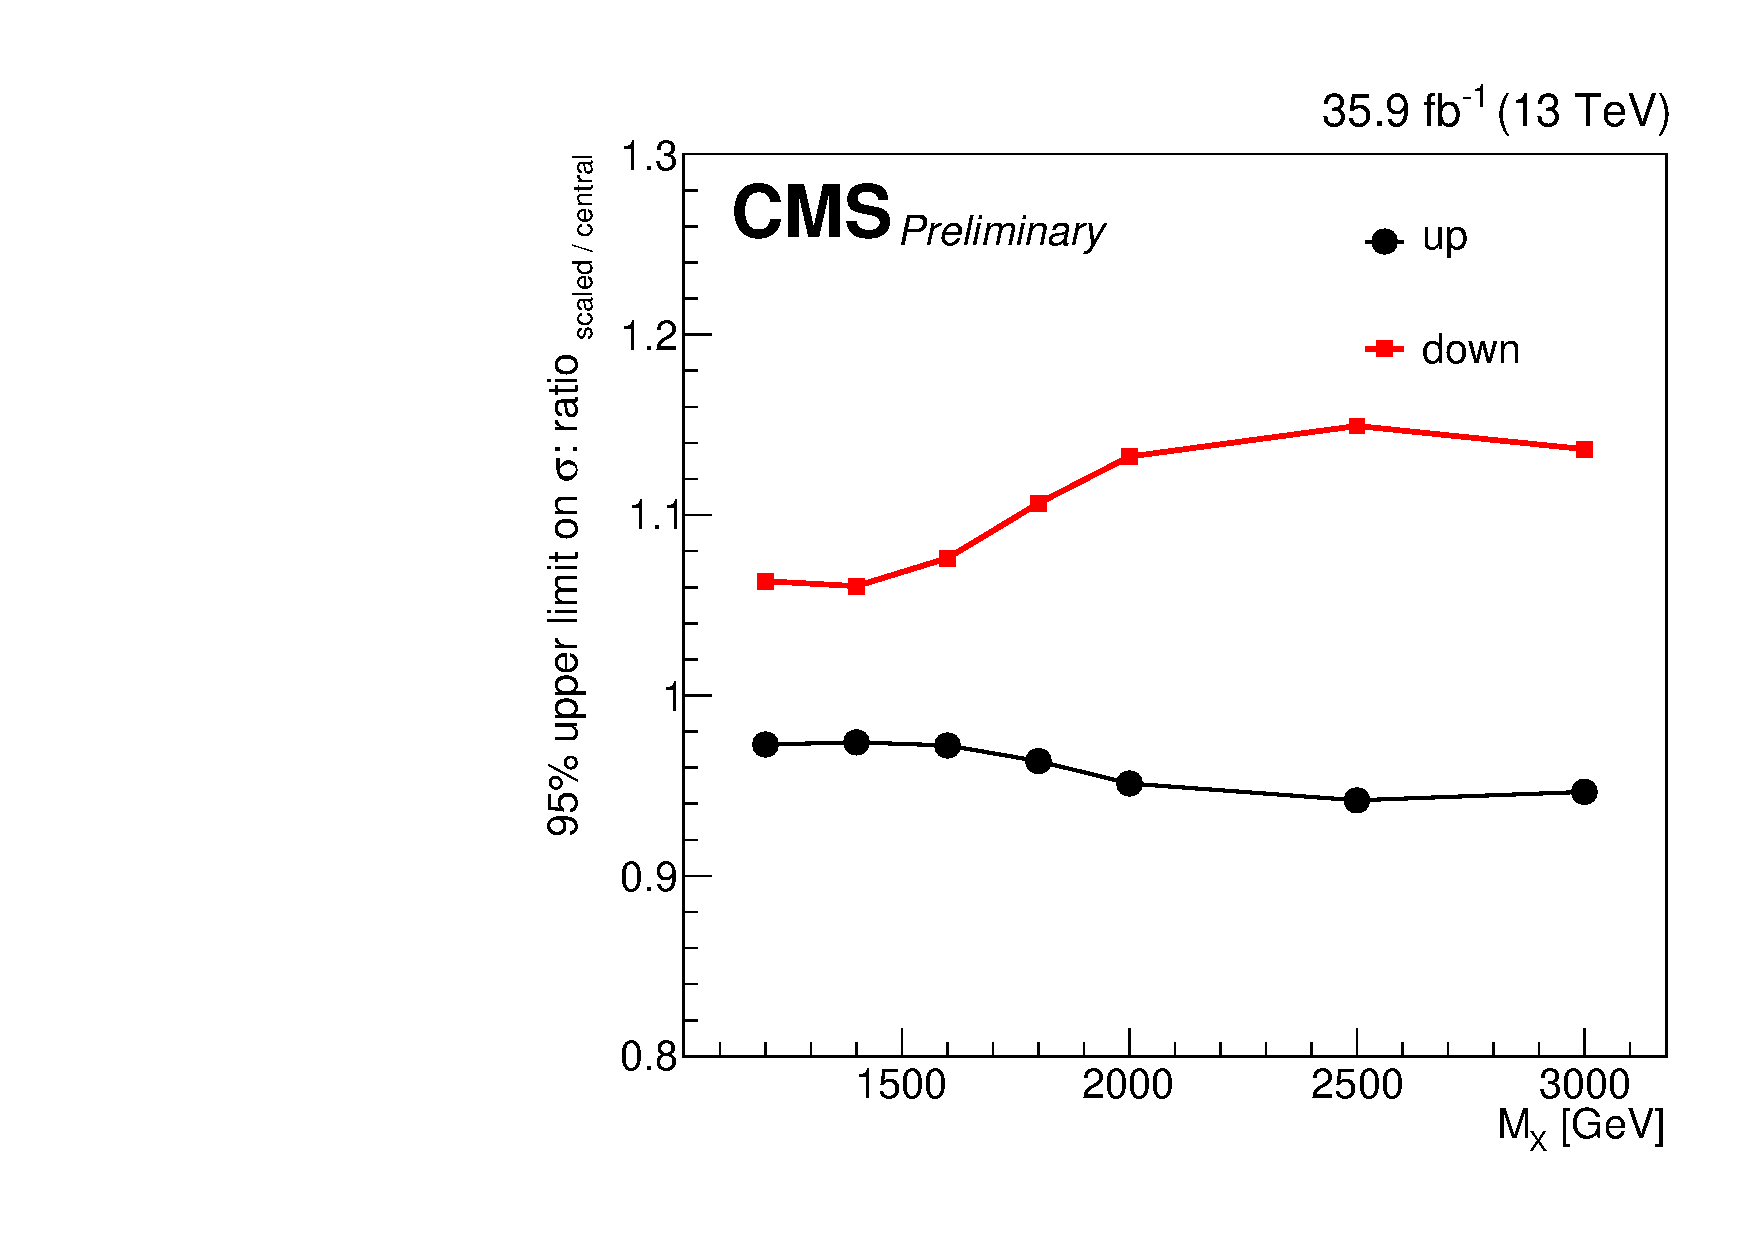
\includegraphics[width=0.5\textwidth]{Figures/plots_uncert/btag_LL.pdf} \\
  \end{tabular}
  \caption{The double-b tagger uncertainty. The scale-up and scale-down to central ratio based on the change of the upper limit are shown in TT (left) and LL (right) category.}

\end{figure}    
  
%https://twiki.cern.ch/twiki/bin/viewauth/CMS/JetWtagging
  \item $\tau _{21}$ scale factor: The uncertainty of $\tau _{21}$ scale factor is measured by JME POG on the samples of semi-leptonic $t\bar{t}$ which is a generous source of W boson. The uncertainty of scale factor in the region $\tau _{21} <$ 0.55 is 14$\% $ per jet~\citep{WTagTWikiWPs}.
 
%https://twiki.cern.ch/twiki/bin/view/CMS/JetResolution#Smearing_procedures 
  \item Jet energy resolution: The procedure is to smear the energy resolution of AK8 jets of simulation as same as those of data~\citep{JER}. 
  
  \item Parton distribution function, PDF: The parton distribution function is a prabability density function of the energy of partons in a proton. The PDF is obtained only by experimental results. There are many sets of PDF trying to well describe them. In CMS, the NNPDF3.0 is used as default PDF set~\citep{Ball:2014uwa}. The uncertainty is derived from the ratio of RMS of the distribution of 100 efficiency by change the weight of different PDFs to the efficiency of the central PDF set. 
	
	\item Factorization scale: the factorization is the energy determining separate the regimes of perturbative and non-perturbative of QCD. The uncertainty is measured the changes of the efficiency by scaling the energy by two or by 0.5.
  
  \begin{figure}[t]
  \centering
 \begin{tabular}{cc}
    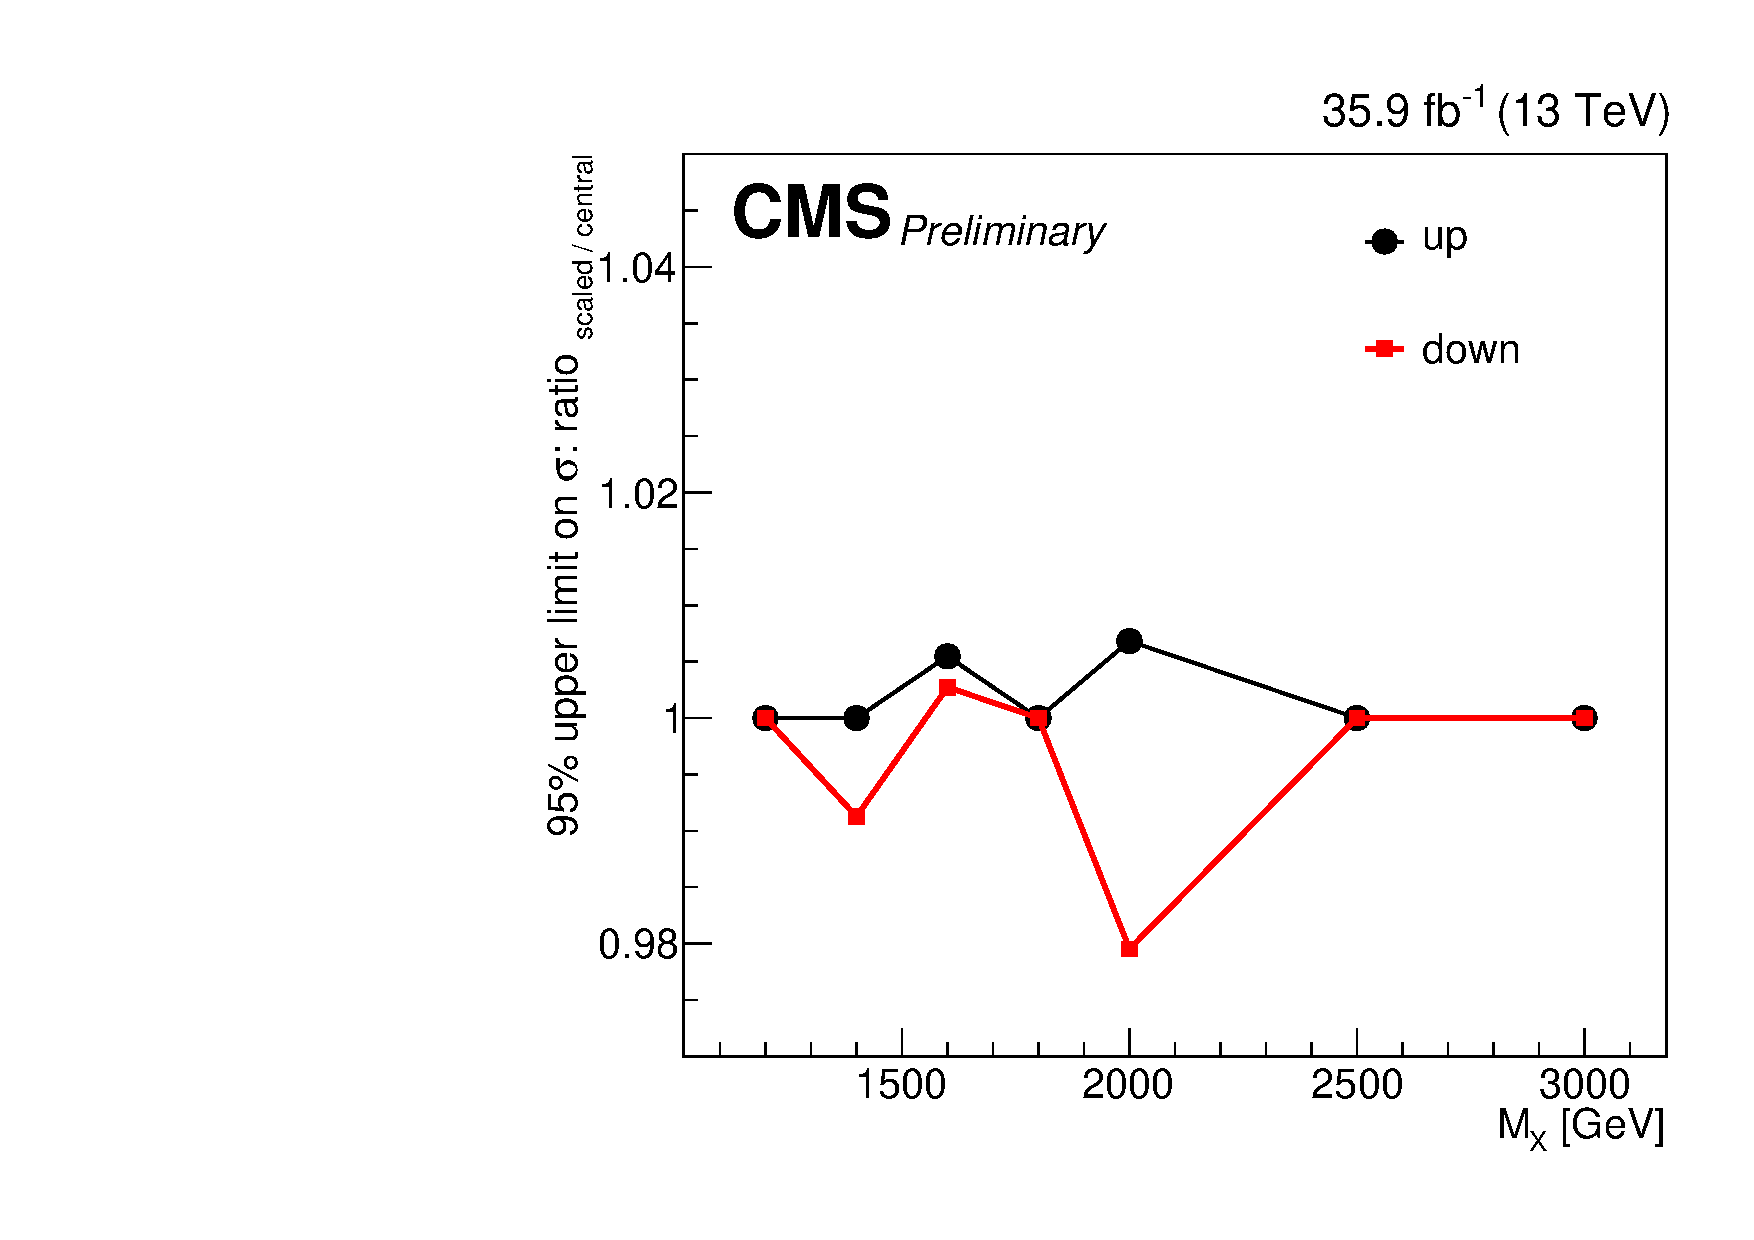
\includegraphics[width=0.5\textwidth]{Figures/plots_uncert/JER_TT.pdf} &
   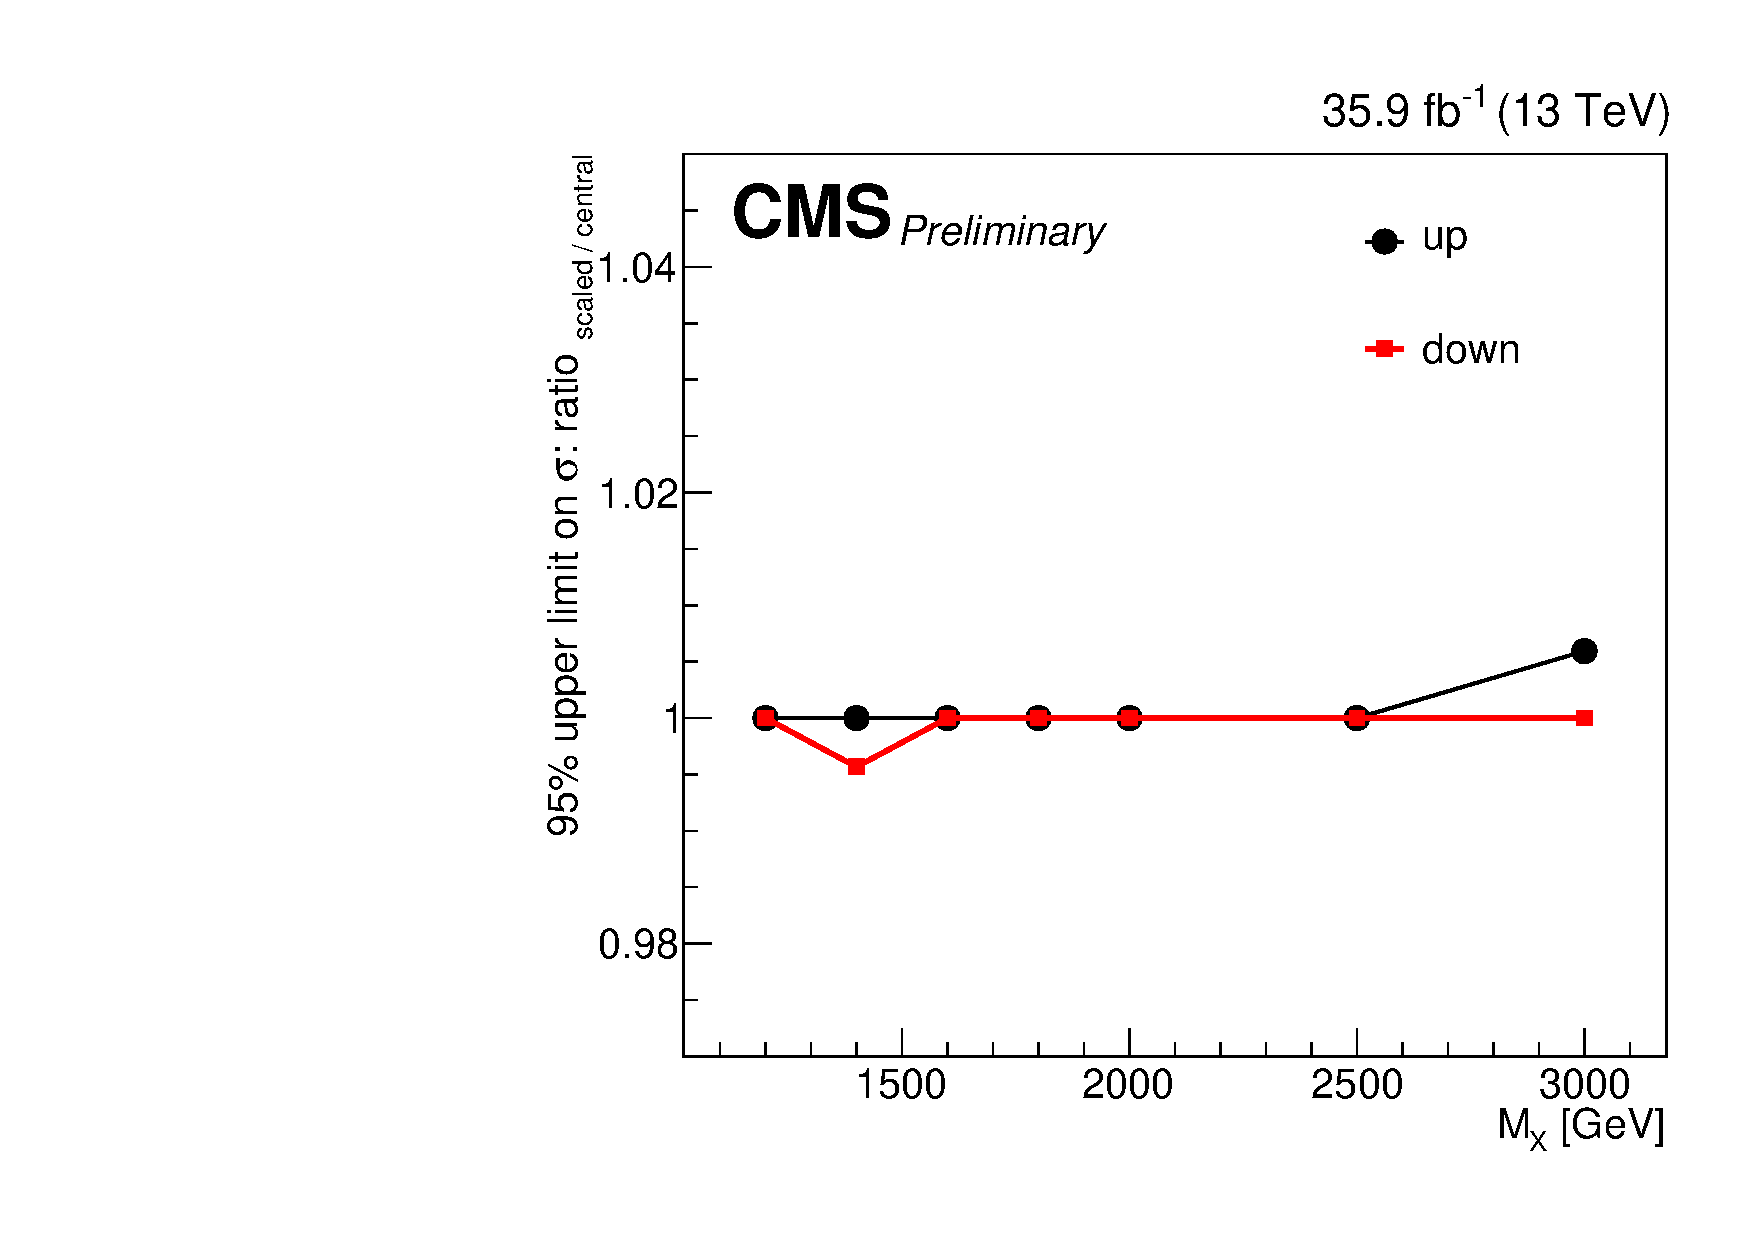
\includegraphics[width=0.5\textwidth]{Figures/plots_uncert/JER_LL.pdf} \\
  \end{tabular}
  \caption{The jet energy resolution uncertainty. The scale-up and scale-down to central ratio based on the change of the upper limit are shown in TT (left) and LL (right) category.}

\end{figure}  
  \item Jet energy scale: The procedure is to weight the four momenta of AK8 jets of simulation as same as those of data~\citep{Chatrchyan:2011ds}. The scale is to calibrate the energy response in ECAL of the jets using $\\gamaa$/Z + jets control samples because the energy of photon, of Z $\rightarrow e^+e^-$ and of Z $\rightarrow \mu^+\mu^-$is measured accurately in ECAL.
  
  \begin{figure}[t]
  \centering
 \begin{tabular}{cc}
    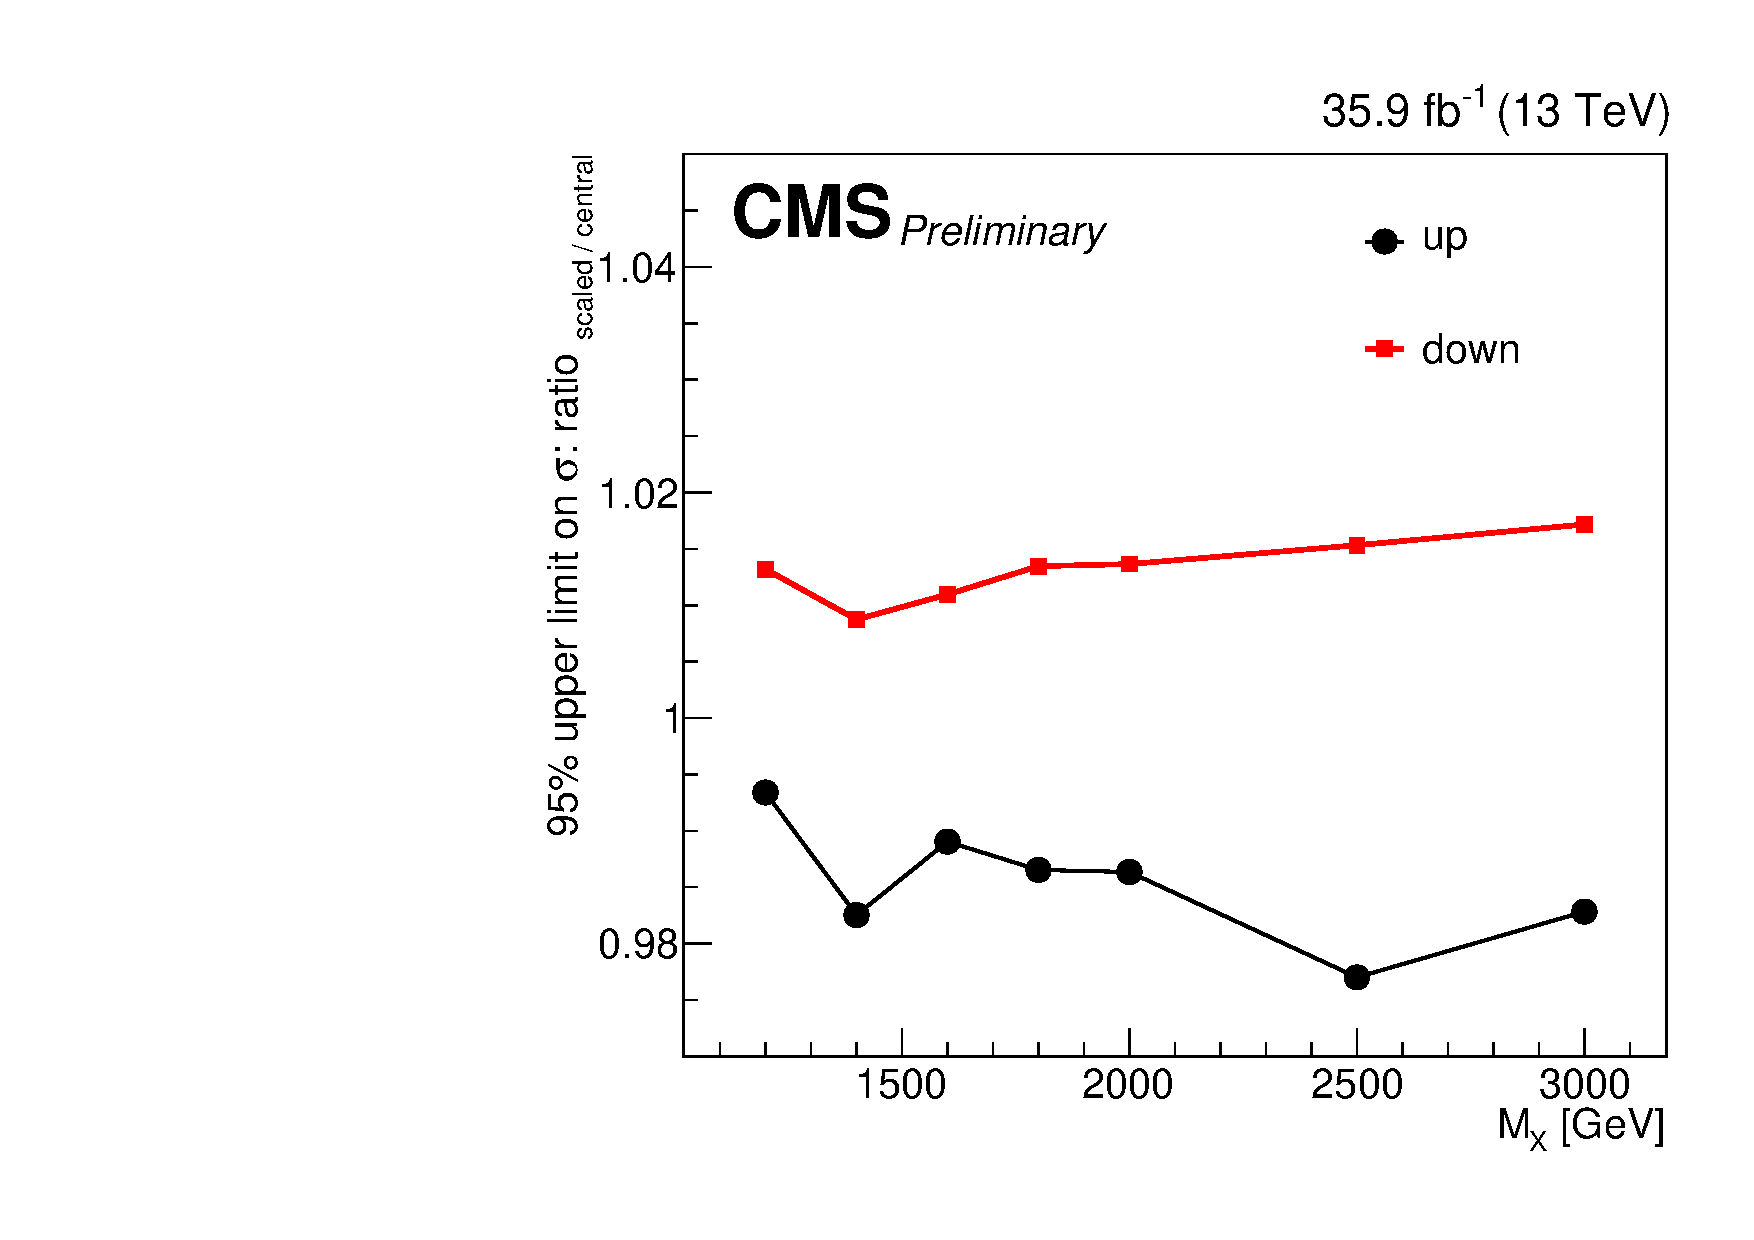
\includegraphics[width=0.5\textwidth]{Figures/plots_uncert/JEC_TT.pdf} &
   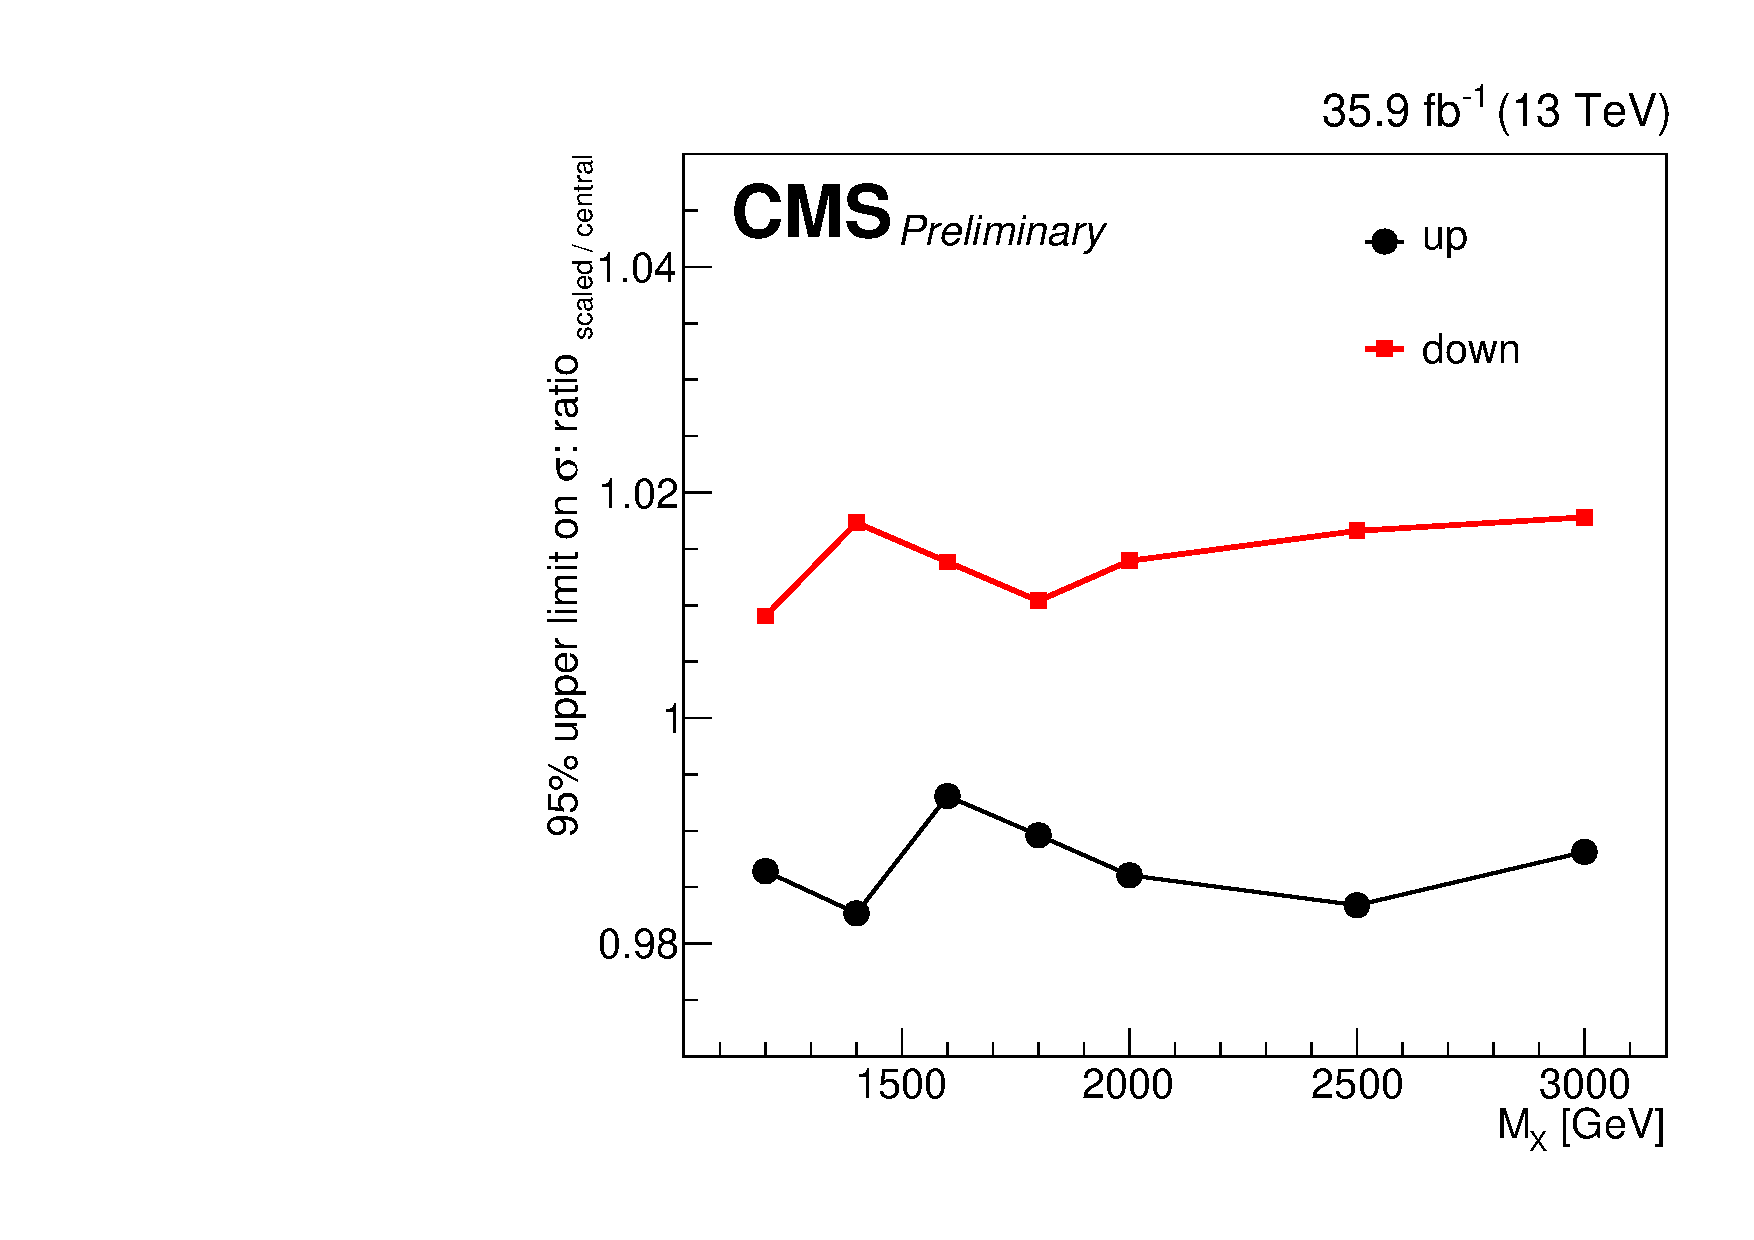
\includegraphics[width=0.5\textwidth]{Figures/plots_uncert/JEC_LL.pdf} \\
  \end{tabular}
  \caption{The jet energy scale uncertainty. The scale-up and scale-down to central ratio based on the change of the upper limit are shown in TT (left) and LL (right) category.}

\end{figure} 

 \begin{figure}[t]
  \centering
 \begin{tabular}{cc}
    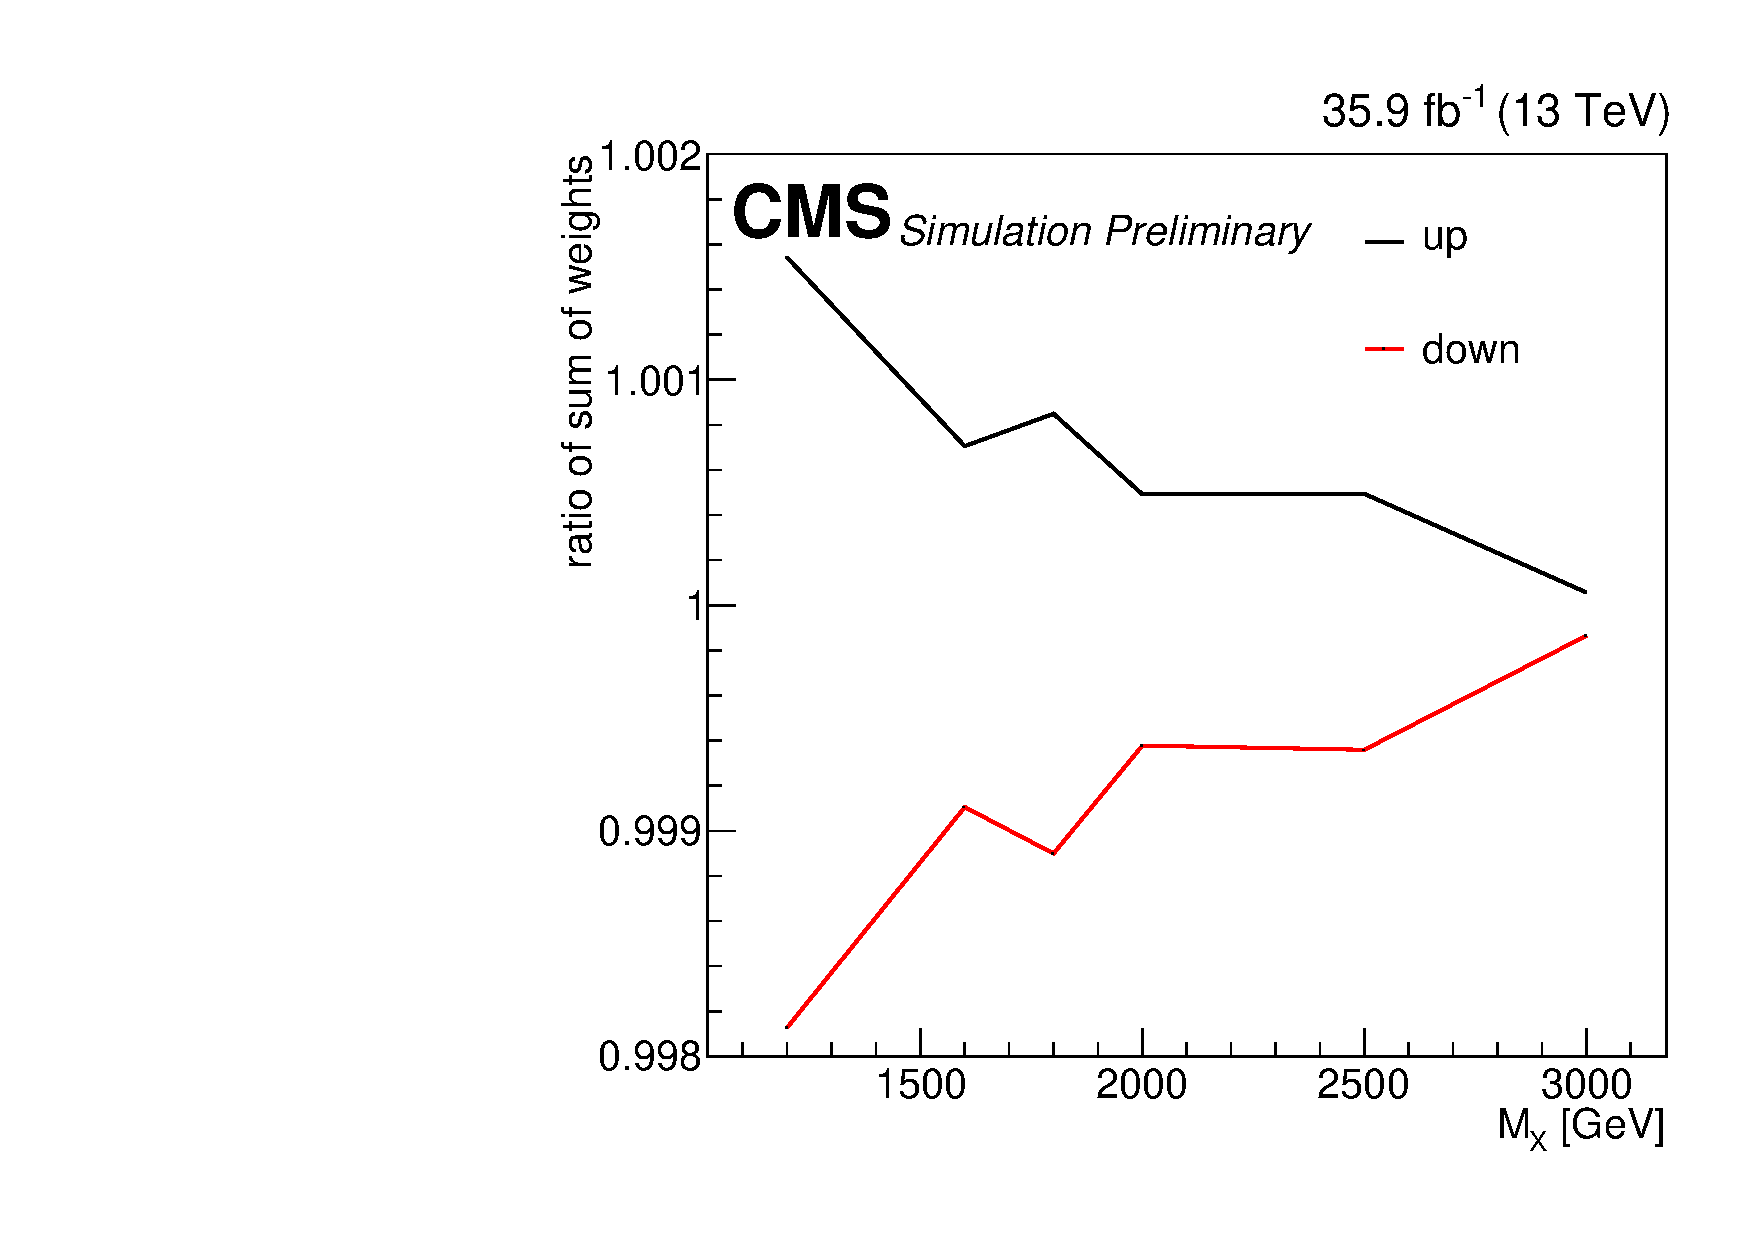
\includegraphics[width=0.5\textwidth]{Figures/scl/scl_TT.pdf} &
   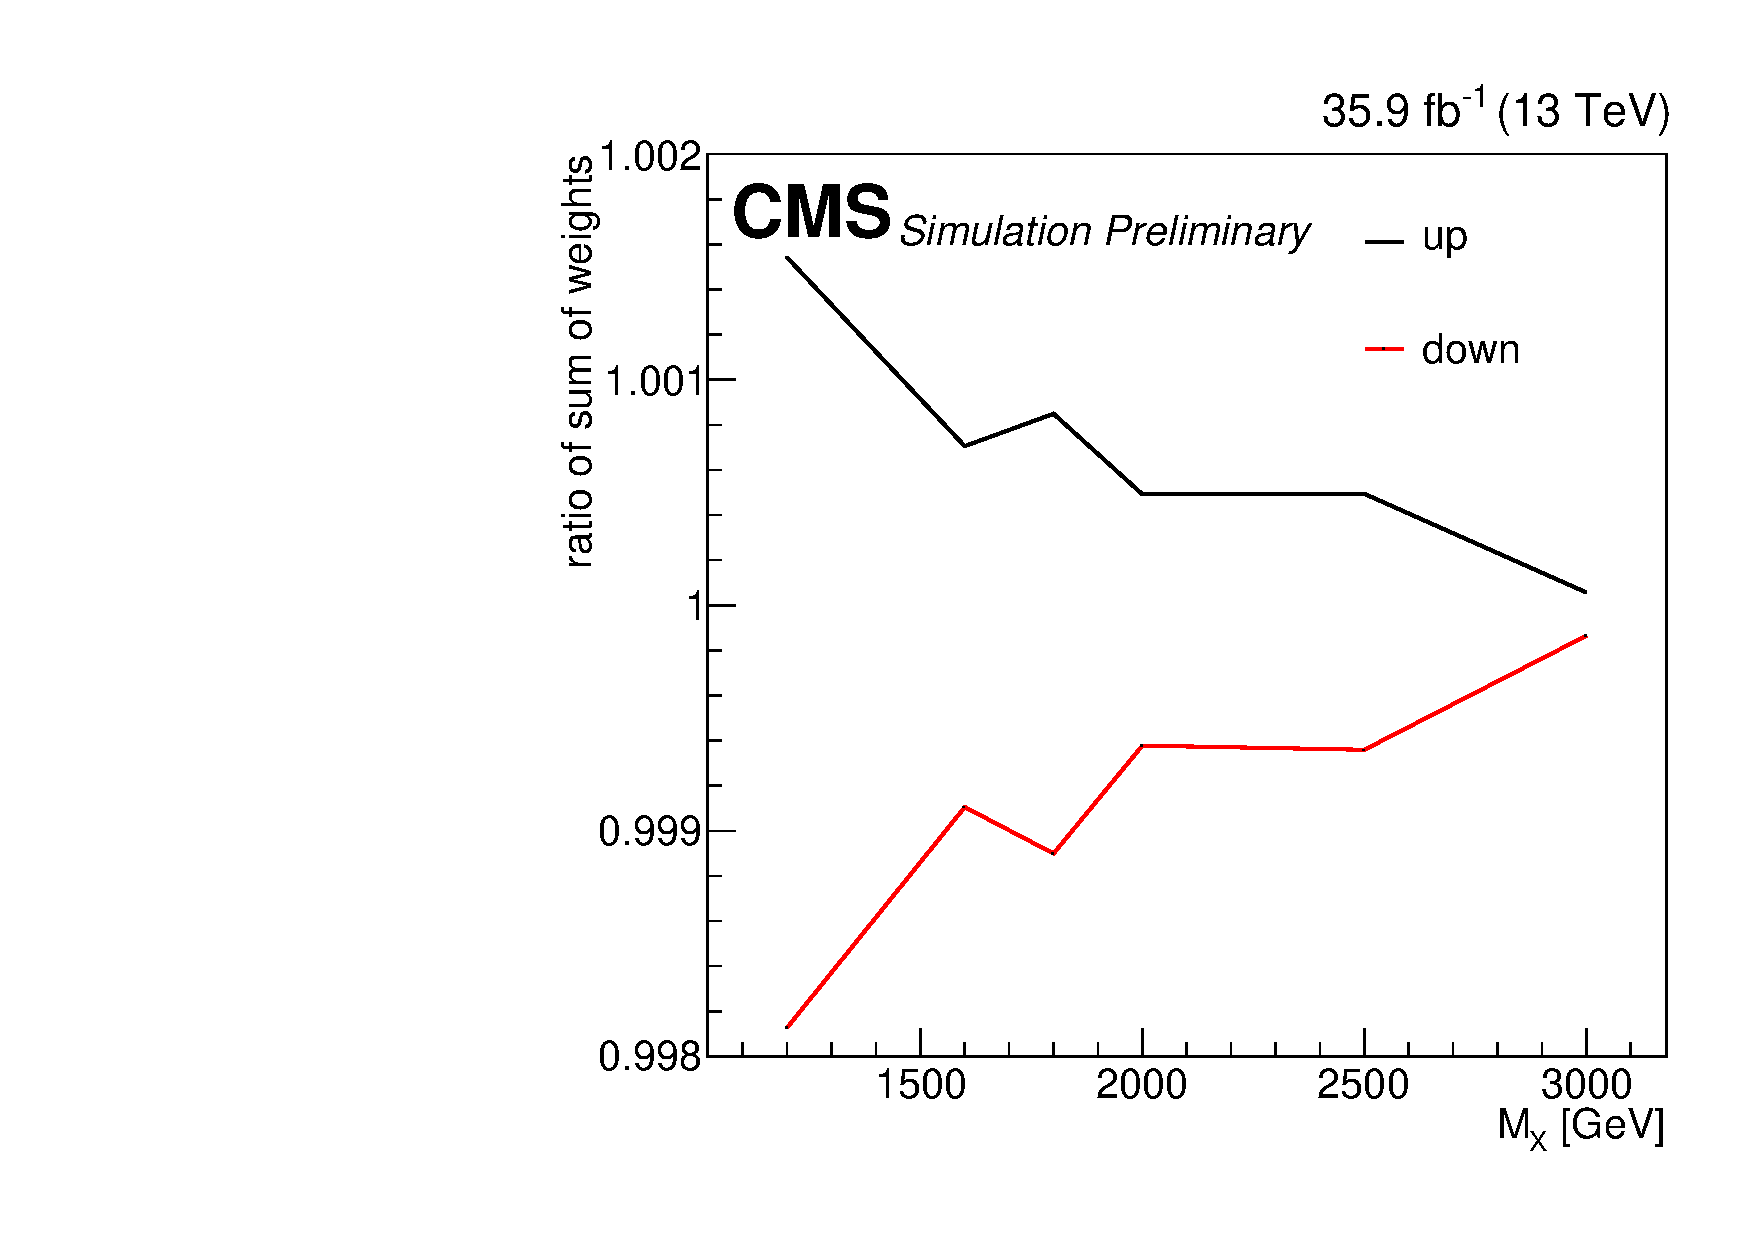
\includegraphics[width=0.5\textwidth]{Figures/scl/scl_TT.pdf} \\
  \end{tabular}
  \caption{The Factorization uncertainty. The scale-up and scale-down to central ratio based on the change of the efficiency are shown in TT (left) and LL (right) category.}

\end{figure} 

 \begin{figure}[t]
  \centering
 \begin{tabular}{cc}
    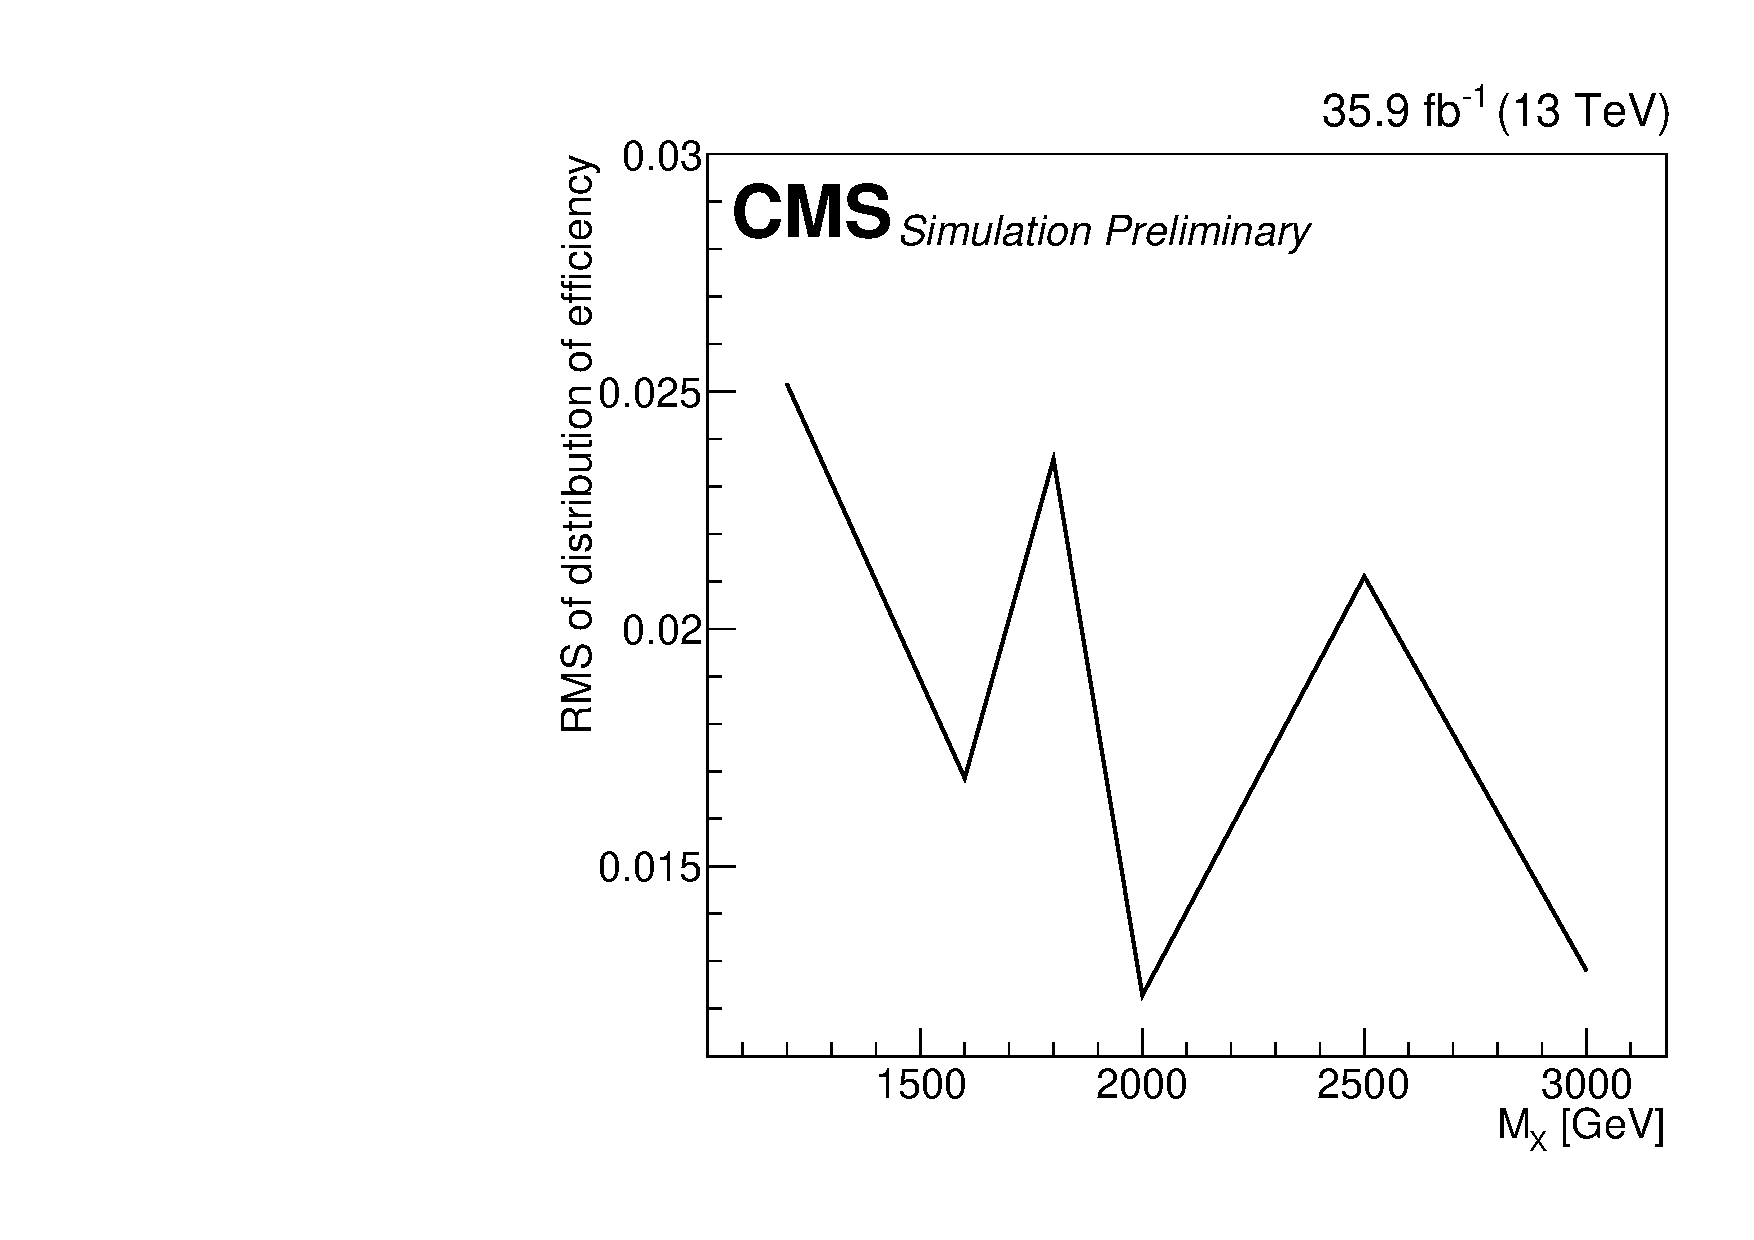
\includegraphics[width=0.5\textwidth]{Figures/eff/uncert_pdf_eff_TT.pdf} &
   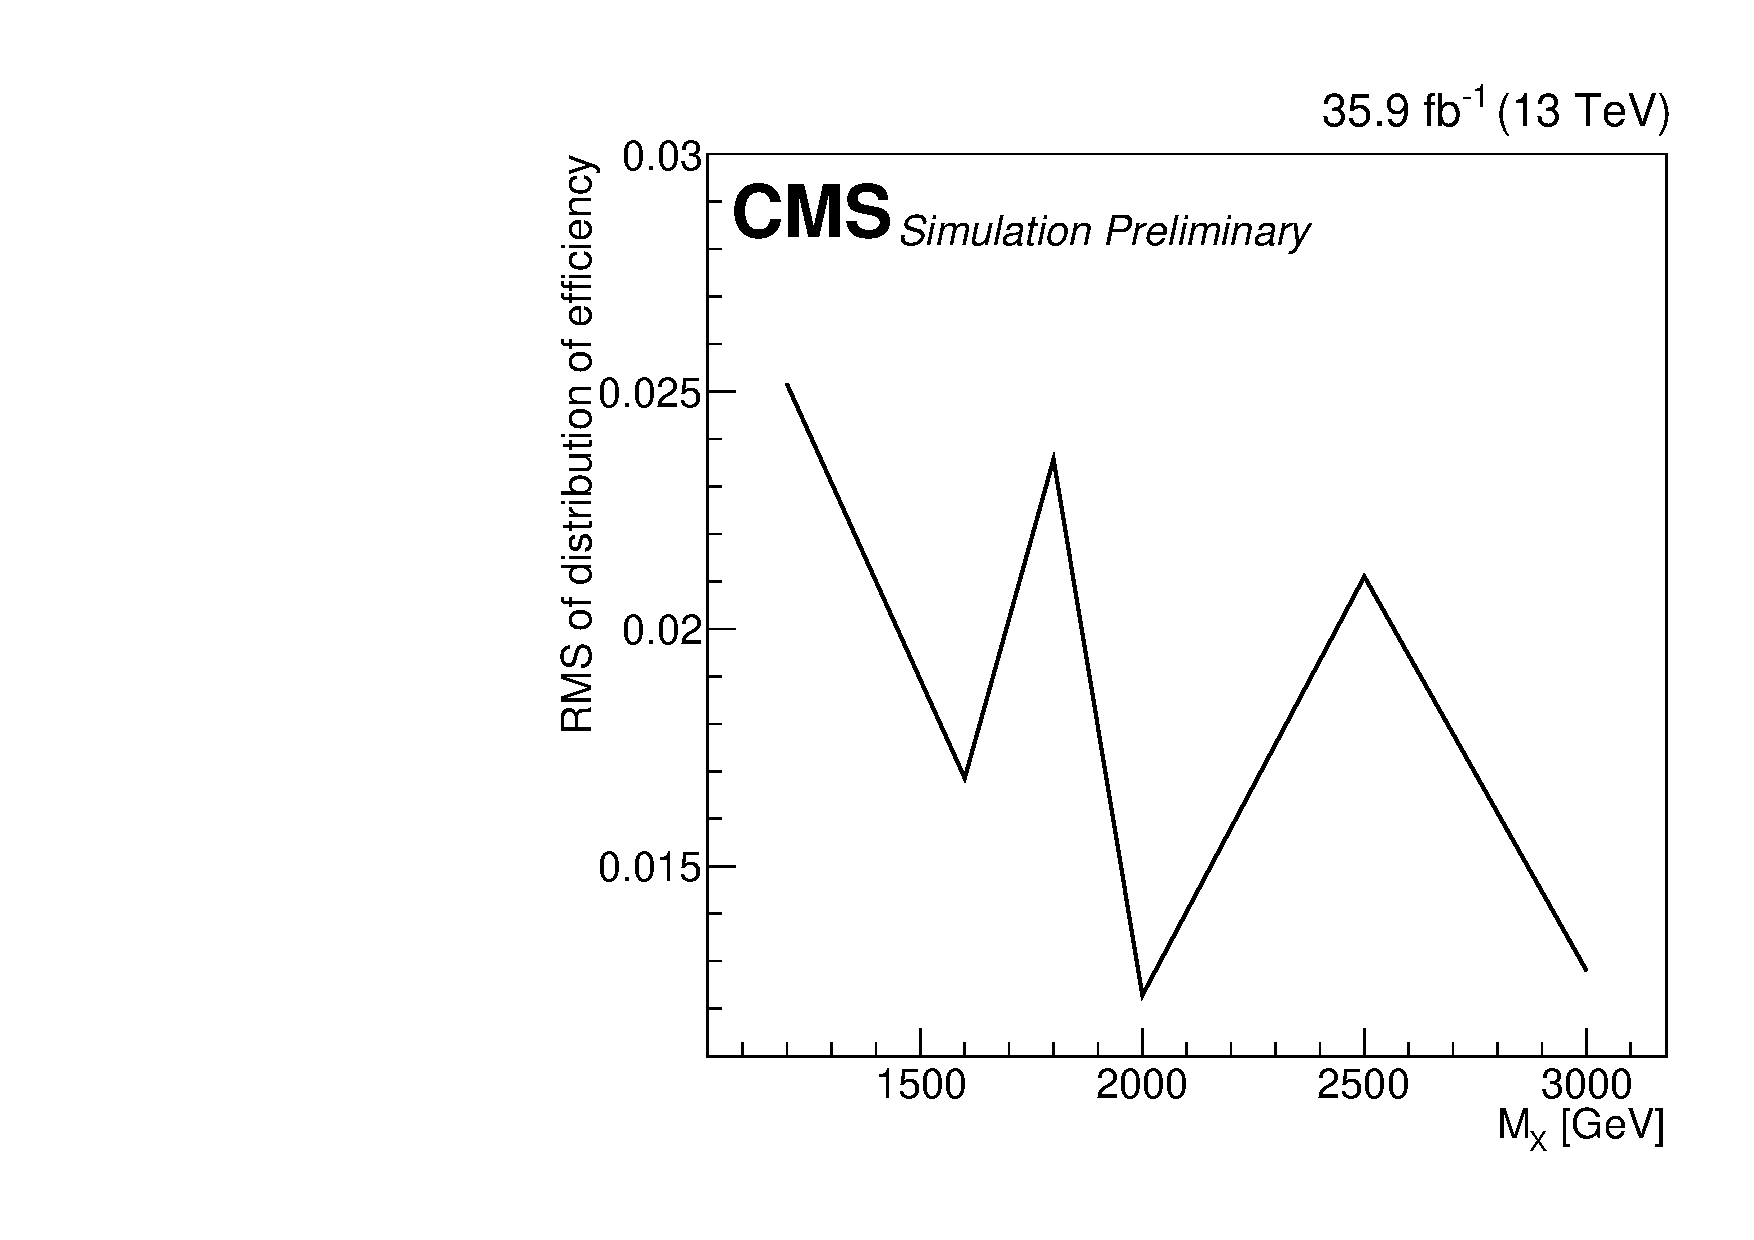
\includegraphics[width=0.5\textwidth]{Figures/eff/uncert_pdf_eff_TT.pdf} \\
  \end{tabular}
  \caption{The jet energy scale uncertainty. The values of ratio RMS of efficiency from 100 p.d.f. sets to efficiency of central value are shown in TT (left) and LL (right) category.}

\end{figure}  

	\item Trigger efficiency scale factor: the trigger efficiency scale factor is measured by the ratio of the efficiency of simulation to that of data. Since we veto the leptonic events, we use JetHt dataset instead of SingleMuon dataset to measure the efficiency of data. The uncertainty comes from propagating the statistic uncertainty added by $\frac{1-efficiency_{PFJET260,QCD}}{efficiency_{pre-selection}}$.The pre-selection is listed:
   \begin{itemize}
	\item Two leading AK8 jets have $p_{T} >$ 300 GeV and |$\eta$| $<$2.4.
	\item 105 $<$ corrected PUPPI soft-drop mass $<$ 135.
	\item $\Delta \eta$(two leading AK8 jets) $<$ 1.3.
	\end{itemize}
	The trigger efficiency scale factor effects less in the analysis because the $M_{jj}$ of the signal is  in the turn-on region where the scale factor is one.
	
\end{itemize}


\clearpage
\section{Summary table}
The summary of all systematic uncertainties is in table 5.1. It also concludes the variation form the uncertainties is considered.
\begin{table}[h!]
  \begin{center}
    \begin{tabular}{l|l|l|l}
    Uncertainty & value(TT) & value(LL) \\
    \hline
    Luminosity &  2.5$\% $ & 2.5$\% $\\
    Pile-up & 1$\% $ & 1$\% $\\
    Jet Energy Resolution &  1$\% $ & 0.5$\% $\\
    Jet Energy Scale &  2$\% $ & 2$\% $\\
    Double-b tagger &  20$\% $ at most & 15$\% $ at most\\
    Higgs tagging & 13-19$\% $ &13-19$\% $ \\
    trigger &  less than 0.1$\% $ & less than 0.1$\% $\\
    $\tau _{21}$ scale factor &  14$\% $ per jet & 14$\% $ per jet\\
    PDF &  2.5$\% $ & 2.5$\% $\\
    scale &  0.2$\% $ & 0.2$\% $\\
    \hline
    \end{tabular}
  \end{center}

  \caption{List of systematic uncertainties and their values.}
\end{table} 